\documentclass[11pt, a4paper]{article} %or article has only section and below, book and report also have chapter: http://texblog.org/2007/07/09/documentclassbook-report-article-or-letter/

\usepackage[utf8]{inputenc}  % use utf8 encoding of symbols such as umlaute for maximal compatibility across platforms

\usepackage{caption}				% provides commands for handling caption sizes etc.
%\usepackage[a4paper, left=25mm, right=20mm, top=25mm, bottom=20mm]{geometry}		 % to easily change margin widths: https://www.sharelatex.com/learn/Page_size_and_margins

\usepackage{etoolbox}    % for conditional evaluations!
\usepackage[bottom]{footmisc}  % I love footnotes! And they should be down at the bottom of the page!
\usepackage{graphicx}        % when using figures and alike
\usepackage[hidelinks]{hyperref}		% for hyperreferences (links within the document: references, figures, tables, citations)

\usepackage{euler}     % a math font, only for equations and alike; call BEFORE changing the main font; alternatives: mathptmx, fourier, 
%\usepackage{gentium} % for a different font; you can also try: cantarell, charter, libertine, gentium, bera, ... http://tex.stackexchange.com/questions/59403/what-font-packages-are-installed-in-tex-live

%------------------------------------------------------------------------------------------------------
%------- text size settings --------------
\setlength{\textwidth}{16cm}% 
\setlength{\textheight}{25cm} %23 
%(these values were used to fill the page more fully and thus reduce the number of pages!)
\setlength{\topmargin}{-1.5cm} %0
\setlength{\footskip}{1cm} %
%\setlength{\hoffset}{0cm} %
\setlength{\oddsidemargin}{0cm}%
\setlength{\evensidemargin}{0cm}%
\setlength{\parskip}{0cm} % Abstand zwischen Absätzen
% ----------------------------------------------------------------
\renewcommand{\textfraction}{0.1} % allows more space to graphics in float
\renewcommand{\topfraction}{0.85}
%\renewcommand{\bottomfraction}{0.65}
\renewcommand{\floatpagefraction}{0.70}


\frenchspacing %http://texwelt.de/wissen/fragen/1154/was-ist-french-spacing-was-macht-frenchspacing
%------------------------------------------------------------------------------------------------------
%------------------------------------------------------------------------------------------------------

\usepackage{Sweave}
\begin{document}
<<<<<<< HEAD
\SweaveOpts{concordance=TRUE}
=======
\Sconcordance{concordance:Knitr-Main.tex:Knitr-Main.Rnw:%
1 40 1 49 0 1 6 90 1 3 0 59 1 3 0 16 1}

>>>>>>> 7e996ed24050650938a643b93597870d6fa79fb8
%\SweaveOpts{concordance=TRUE}
%%%%%%%%%%%%% this bit is new to Knitr: %%%%%%%%%%%%%%%%%%%%%


\title{A tutorial for Step Selection Function}

\author{P. Antkowiak\thanks{M.Sc. programme "GIS und Umweltmodellierung" at University of Freiburg} \and H. Tripke\thanks{M.Sc. programme "Wildlife, Biodiversity and Vegetation" at University of Freiburg} \and C. Wilhelm\thanks{M.Sc. programme "Wildlife, Biodiversity and Vegetation" at University of Freiburg}}
% for more control, multiple affiliations, line breaks and alike, use the authblk package!!

\date{\today} % !!use package isodate for more control of date formatting!!

\maketitle

%------------------------------------------------------------------------------------------------------
%------------------------------------------------------------------------------------------------------

\tableofcontents

\newpage

\section{Introduction}%------------------------------------------------------------------------------------------------------

In addition to Resources Selection Functions (RSF) another powerful tool for evaluating data on animal movements and habitat selection are Step Selection Functions (SSF). The latter are used to estimate resource selection by comparing observed habitat use with available structures. Given GPS locations of a collared individual each observation is connected by a linear segment. These segments are considered as steps. The time intervals influencing the step length should be choosen carefully (i.e. by conducting a pilot study) to meet the requirements of the study questions and the target species. The SSF than calculates random steps by taking measured angle and distance along steps and using the observed positions as starting points. These alternative steps represent the available habitat within a realistic step length of the observed positions. Finally, we can compare spatial attributes on  both and test for effects that explain habitat selection by animals \cite{thurfjell2014applications}.\\ So far, SSF models were mainly done using Geospatial Modelling Environment (GME) that works with a GIS\footnote{www.spatialecology.com/gme/}. However, more and more packages for analyzing animal movements are provided in R. Non of these packages is designed for doing a SSF only but quite a number provide already helpful functions to perform single steps of the Selection Function. Therefore, the aim of this tutorial is to collect all functions necessary to conduct a SSF and order them in a  way that intuitively makes you understand how to run a SSF with your own data. Each step will be explained using an exemplary dataset of GPS locations collected from seven Cougars (\textit{Puma concolor}) in the year 2010 (in the following adressed as \texttt{xmpl}).\\


Figure~\ref{fig:Flowchart} provides an overview of all necessary steps and potential options to conduct a SSF. This tutorial will guide you through each step and gives brief instructions on how to implement the functions and what to consider beforehand.
To conduct a SSF using this tutorial we need you to store your initial data  in two independant datasets: \begin{enumerate} \item {A raster file of your spatial attributes (\emph{Raster data})} and \item{GPS locations of your individuals assigned with a time stamp (\emph{Waypoint data})}. \end{enumerate} 
We will start with the \emph{Waypoint data} because these need to transformed a couple of times to be able to work with them. You can find the single steps on the right site of Figure~\ref{fig:Flowchart}. After loading the table into R you need to create an so-called \texttt{ltraj} object. This data class can now be further transformed by ... Random steps should only be calculated for equal time intervals. These can be defined by creating bursts. Each burst has an unique ID (often including an ID for the individual and the time stamp). While there are many options to adjust your \emph{Waypoint data} the \emph{Raster data} describing your spatial attributes needs not much of change. Once you created random steps for your observed positions you can extract the spatial attributes for each of those positions by using the function \texttt{extract}. At this point \emph{Waypoint} and \emph{Raster data} will be combined and your final model can be written.   


DO WE NEED A EQUATION??
\[
\displaystyle w(x) = exp(\beta1 x1 + \beta2x2 + ... + \beta p xp)
\]
\
Why did we not use the data (Wildboar) prepared for the adehabitatLT package? - No information on details, metadata provided, it is hard to understand when to use which dataset and why.



\begin{figure} % you can (but shouldn't) use [h] behind {figure} to force the picture to go here. However, the idea of LaTeX is that it will do things for you, so too much interfering is not saving you any time.
% see also here: http://en.wikibooks.org/wiki/LaTeX/Floats,_Figures_and_Captions#Captions
\captionsetup{width=1\textwidth}
\centering
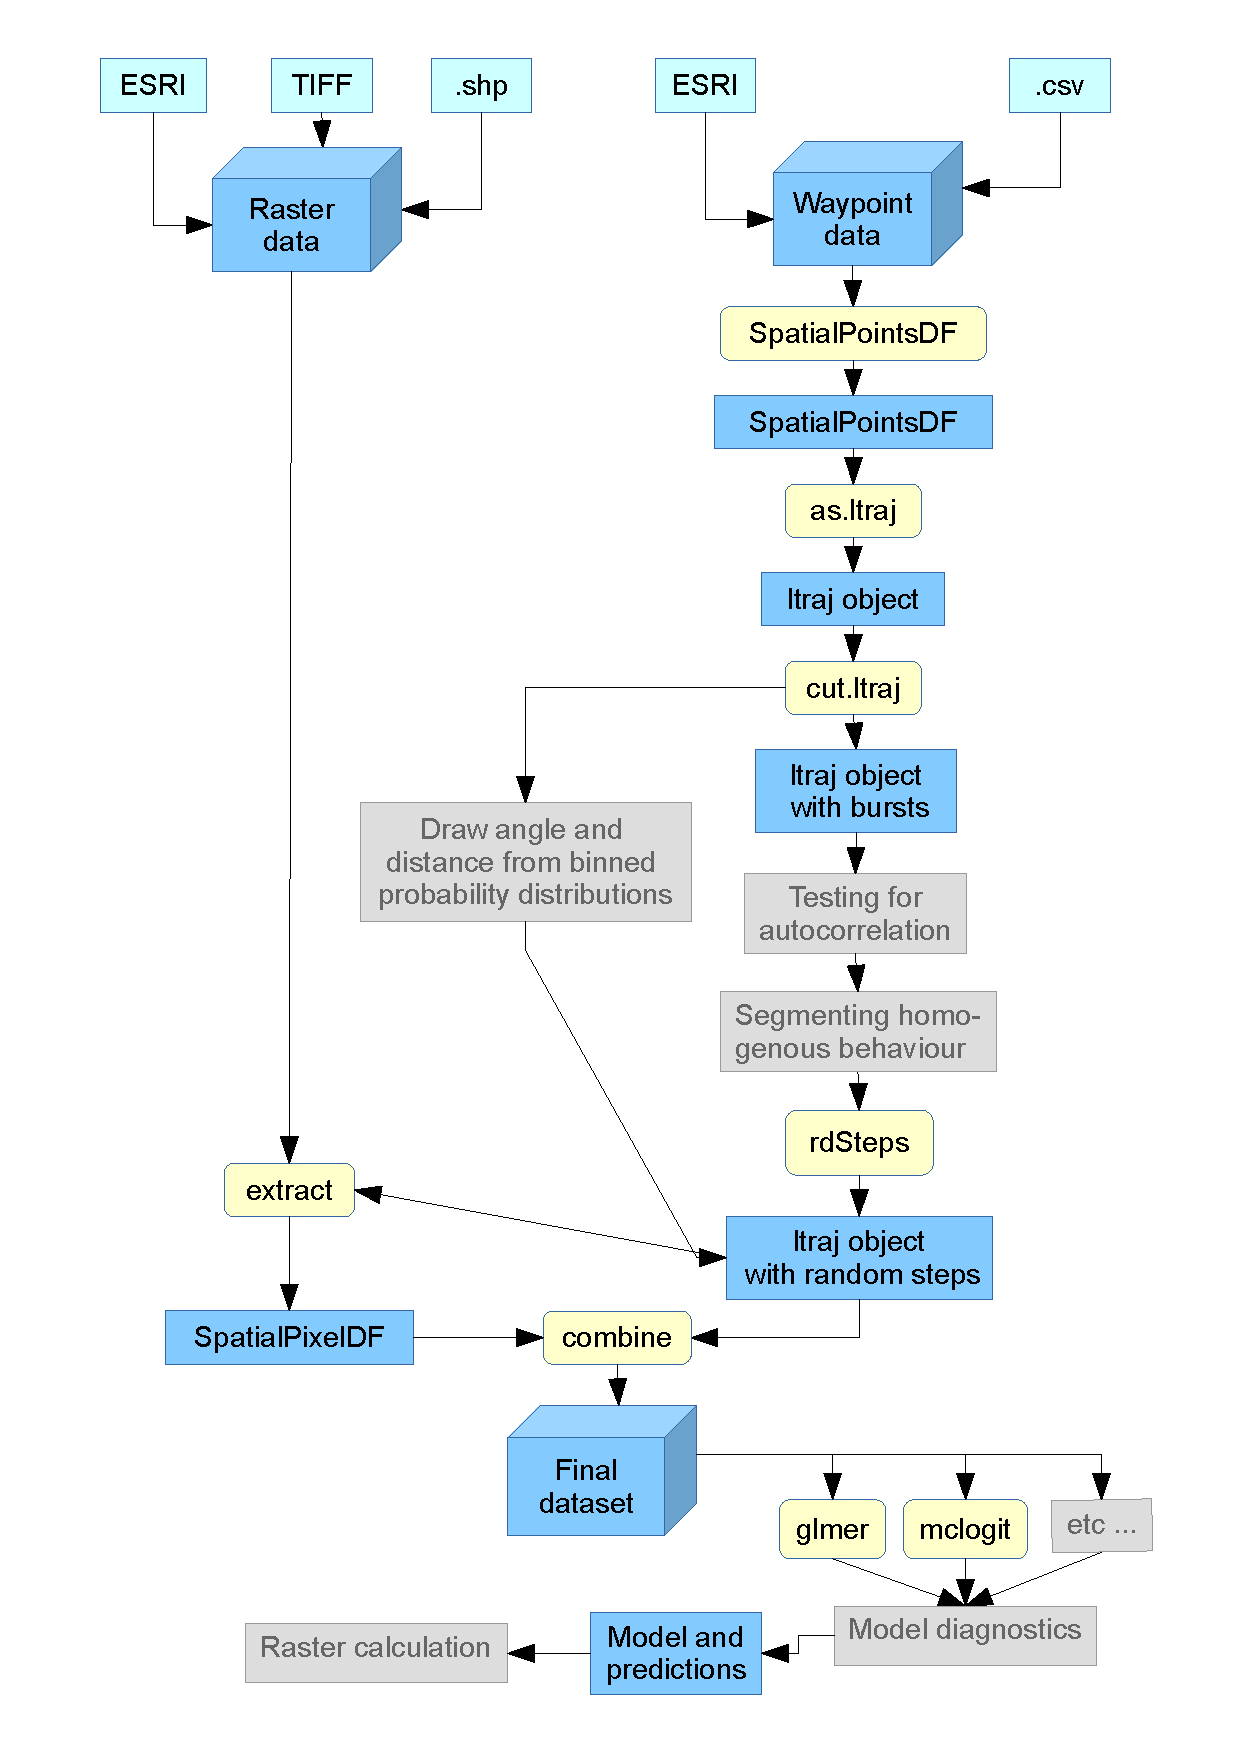
\includegraphics[width=1\textwidth]{Flowchart.pdf} %our perfect workflow!
\caption{Conducting a Step Selection Function using existing R-packages. The yellow boxes show the name of the fucntion applied while the blue boxes provide the type of object or data. Following the arrows a step by step instruction is provided ...}
\label{fig:Flowchart}
\end{figure}




\subsection{Preparations}
Before you can actually start using the tutorial for conducting SSF you need to load a bunch of packages in R. Some of them require others so that you have to add all these to your library:

\subsection{Packages - what we need}

<<<<<<< HEAD
\begin{knitrout}
\definecolor{shadecolor}{rgb}{0.969, 0.969, 0.969}\color{fgcolor}\begin{kframe}
\begin{alltt}
\hlcom{# installing packages -----------------------------------------------------}
\hlcom{## for implementing SSF}
\hlcom{# install.packages("adehabitat") # outdated version, not needed for this tutorial}
\hlkwd{install.packages}\hlstd{(}\hlstr{"adehabitatHR"}\hlstd{)}
\hlkwd{install.packages}\hlstd{(}\hlstr{"adehabitatHS"}\hlstd{)}
\hlkwd{install.packages}\hlstd{(}\hlstr{"adehabitatLT"}\hlstd{)}
\hlkwd{install.packages}\hlstd{(}\hlstr{"adehabitatMA"}\hlstd{)}
\hlkwd{install.packages}\hlstd{(}\hlstr{"tkrplot"}\hlstd{)}
\hlkwd{install.packages}\hlstd{(}\hlstr{"hab"}\hlstd{,} \hlkwc{repos} \hlstd{=} \hlstr{"http://ase-research.org/R/"}\hlstd{)} \hlcom{# regular}
\hlkwd{install.packages}\hlstd{(}\hlstr{"hab"}\hlstd{,} \hlkwc{repos} \hlstd{=} \hlstr{"http://ase-research.org/R/"}\hlstd{,} \hlkwc{type} \hlstd{=} \hlstr{"source"}\hlstd{)} \hlcom{# for self-compiling}

\hlcom{# for handling ratser data}
\hlkwd{install.packages}\hlstd{(}\hlstr{"move"}\hlstd{)}
\hlkwd{install.packages}\hlstd{(}\hlstr{"raster"}\hlstd{)}
\hlkwd{install.packages}\hlstd{(}\hlstr{"rgdal"}\hlstd{)}
\hlcom{#install.packages("")}

\hlcom{# loading the packages}
\hlcom{# require(adehabitat) # keep fingers off this package. It is outdated.}
\hlkwd{require}\hlstd{(hab)}
\hlkwd{require}\hlstd{(adehabitatMA)}
\hlkwd{require}\hlstd{(adehabitatHR)}
\hlkwd{require}\hlstd{(adehabitatHS)}
\hlkwd{require}\hlstd{(adehabitatLT)}


\hlcom{## for i dont know}

\hlcom{#require(move)}
\hlcom{#require(raster)}
\hlcom{#require(rgdal)}
\hlcom{#require(tkrplot)}
\hlcom{#require(raster)}
\hlcom{#require(sp)}
\end{alltt}
\end{kframe}
\end{knitrout}

\section{All right site steps}

\subsection{Load telemetry data (*.csv, ESRI)}%------------------------------------------------------------------------------------------------------
The data for the analysis should be safed in a simple *.csv format. Depending on your analysis you have to include 
\begin{enumerate}
\item{coordinates}
\item{ID}
\item{date and/or time}
\item{...}
\end{enumerate}



\subsection{Create a Spatial Points Data Frame}%------------------------------------------------------------------------------------------------------

\subsection{Create a ltraj object}%------------------------------------------------------------------------------------------------------
 

\subsection{Compute random steps}

The function \textbf{rdSteps} removes the first and the last data point. That's what you want. 

\section{Spatial covariates}%----------------------------------------------------------------------------------------------------------------------------
This section explains the use of spatial parameters that will be tested for selection by the target species. You should store these data in raster files (probably ESRI (*.adf) or *.tif) and for time reasons already clipped to your area. How you can do this in R please read the GIS instructions from the other group ;)   

\subsection{Load raster data (ESRI, *.tif, (*.shp))}%------------------------------------------------------------------------------------------------------
With a simple function stored in the package \textbf{raster} you are able to upload any ratser file into R. Examplarily we are using the ratser data for ruggedness and canopy cover for the study area.  


\begin{knitrout}
\definecolor{shadecolor}{rgb}{0.969, 0.969, 0.969}\color{fgcolor}\begin{kframe}
\begin{alltt}
\hlcom{#install.packages("RArcInfo")}
\hlcom{#require(RArcInfo)}
\hlkwd{require}\hlstd{(raster)}
\hlkwd{require}\hlstd{(rgdal)}

\hlkwd{require}\hlstd{(sp)}


\hlcom{#?raster}
\hlcom{#getwd()}
\hlcom{#setwd("/home/Peter/")}

\hlstd{ruggedness} \hlkwb{<-} \hlkwd{raster}\hlstd{(}\hlstr{"/home/Peter/Dokumente/uni/WS_14_15/Best Practice R/Dataset/NEW GIS LAYERS/tri1/w001001.adf"}\hlstd{)}
\hlcom{# plot(ruggedness) # outcomment this if you just quickly want to run the script. Takes a minute to process.}

\hlstd{landcover} \hlkwb{<-} \hlkwd{raster}\hlstd{(}\hlstr{"/home/Peter/Dokumente/uni/WS_14_15/Best Practice R/Dataset/NEW GIS LAYERS/lc_30/w001001.adf"}\hlstd{)}
\hlcom{# plot(landcover) # outcomment this if you just quickly want to run the script. Takes a minute to process.}

\hlstd{canopycover} \hlkwb{<-} \hlkwd{raster}\hlstd{(}\hlstr{"/home/Peter/Dokumente/uni/WS_14_15/Best Practice R/Dataset/NEW GIS LAYERS/cc_abmt/w001001.adf"}\hlstd{)}
\hlcom{# plot(canopycover) # outcomment this if you just quickly want to run the script. Takes a minute to process.}

\hlstd{disthighway} \hlkwb{<-} \hlkwd{raster}\hlstd{(}\hlstr{"/home/Peter/Dokumente/uni/WS_14_15/Best Practice R/Dataset/NEW GIS LAYERS/disthwy/w001001.adf"}\hlstd{)}
\hlcom{# plot(disthighway) # outcomment this if you just quickly want to run the script. Takes a minute to process.}

\hlstd{distroad} \hlkwb{<-} \hlkwd{raster}\hlstd{(}\hlstr{"/home/Peter/Dokumente/uni/WS_14_15/Best Practice R/Dataset/NEW GIS LAYERS/distsmrd/w001001.adf"}\hlstd{)}
\hlkwd{plot}\hlstd{(distroad)} \hlcom{# outcomment this if you just quickly want to run the script. Takes a minute to process.}
\end{alltt}
\end{kframe}
\end{knitrout}


\subsection{Extract coordinates for comparison of used and random points} %------------------------------------------------------------------------------------------------------
Peter is successfully doing this step!!

<<<<<<< HEAD
\section{Load telemetry data (*.csv, ESRI)}%------------------------------------------------------------------------------------------------------
=======
\begin{Schunk}
\begin{Sinput}
> # installing packages -----------------------------------------------------
> ## for implementing SSF
> # install.packages("adehabitat") # outdated version, not needed for this tutorial
> install.packages("adehabitatHR")
> install.packages("adehabitatHS")
> install.packages("adehabitatLT")
> install.packages("adehabitatMA")
> install.packages("tkrplot")
> install.packages("hab", repos = "http://ase-research.org/R/") # regular
> install.packages("hab", repos = "http://ase-research.org/R/", type = "source") # for self-compiling
> # for handling ratser data
> install.packages("move")
> install.packages("raster")
> install.packages("rgdal")
> #install.packages("")
> 
> # loading the packages
> # require(adehabitat) # keep fingers off this package. It is outdated.
> require(hab)
> require(adehabitatMA)
> require(adehabitatHR)
> require(adehabitatHS)
> require(adehabitatLT)
> 
> 
> ## for i dont know
> 
> #require(move)
> #require(raster)
> #require(rgdal)
> #require(tkrplot)
> #require(raster)
> #require(sp)
> 
\end{Sinput}
\end{Schunk}

\section{All right site steps}

\subsection{Load telemetry data (*.csv, ESRI)}%------------------------------------------------------------------------------------------------------
>>>>>>> 7e996ed24050650938a643b93597870d6fa79fb8
The data for the analysis should be safed in a simple *.csv format. Depending on your analysis you have to include 
\begin{enumerate}
\item{coordinates}
\item{ID}
\item{date and/or time}
\item{...}
\end{enumerate}



\section{Create a Spatial Points Data Frame}%------------------------------------------------------------------------------------------------------

<<<<<<< HEAD
\section{Create a ltraj object}%------------------------------------------------------------------------------------------------------


\section{Creating Bursts}%

For analysing the data, there might be the need to create "sub-bursts" within your trajectory. For example, if the individuals were only recorded during the day, the monitoring took place over two consecutive years or the time lag between the relocations differs remarkably. Looking at those different parts seperately might be necessary for different reasons. The function \texttt{cutltraj} splits the given bursts of your \texttt{ltraj} object into smaller burst according to a specified criterion. In contrast, the function \texttt{bindltraj} combines the bursts of an object of class \texttt{ltraj} with the same attribute "id" to one unique burst. \cite{Package2011} To find out if there are more missing values, you can plot the \texttt{ltraj} object. For that, you need to define the time interval you are looking at. 


In our example, the locations of the cougars were recorded every 3 hours, starting at 3 AM. The location at midnight is always missing. We now want to split the existing bursts (individuals) into "sub-bursts" where the time lag is smaller than 3 hours. To get an impression about the time lags we plotted the different bursts (individuals).

\begin{knitrout}
\definecolor{shadecolor}{rgb}{0.969, 0.969, 0.969}\color{fgcolor}\begin{kframe}
\begin{alltt}
\hlkwd{plotltr}\hlstd{(xmpl.ltr,} \hlstr{"dt/3600"}\hlstd{)}

\hlcom{# time log 1 hour}

\hlkwd{plotltr}\hlstd{(xmpl.ltr,} \hlstr{"dt/3600/3"}\hlstd{)}

\hlcom{# time log 3 hours}
\end{alltt}
\end{kframe}
\end{knitrout}

Because we want to keep relocations which are only a few minutes "wrong", we need a function which defines \texttt{dt}, which is the time interval between successive relocations (measured in seconds).

\begin{knitrout}
\definecolor{shadecolor}{rgb}{0.969, 0.969, 0.969}\color{fgcolor}\begin{kframe}
\begin{alltt}
\hlstd{foo} \hlkwb{=} \hlkwa{function}\hlstd{(}\hlkwc{dt}\hlstd{) \{}\hlkwd{return}\hlstd{(dt}\hlopt{>} \hlstd{(}\hlnum{3800}\hlopt{*}\hlnum{3}\hlstd{))\}}
\end{alltt}
\end{kframe}
\end{knitrout}

Then we split the object of class \texttt{ltraj} according to that function into smaller bursts. The bursts we had before applying this function still remain.

\begin{knitrout}
\definecolor{shadecolor}{rgb}{0.969, 0.969, 0.969}\color{fgcolor}\begin{kframe}
\begin{alltt}
\hlstd{xmpl.cut} \hlkwb{<-} \hlkwd{cutltraj}\hlstd{(xmpl.ltr,} \hlstr{"foo(dt)"}\hlstd{,} \hlkwc{nextr} \hlstd{=} \hlnum{TRUE}\hlstd{)}
\end{alltt}
\end{kframe}
\end{knitrout}

=======
\subsection{Create a ltraj object}%------------------------------------------------------------------------------------------------------
 
>>>>>>> 7e996ed24050650938a643b93597870d6fa79fb8

\section{Compute random steps}

The function \textbf{rdSteps} removes the first and the last data point. That's what you want. 

<<<<<<< HEAD
=======
>>>>>>> fbdcfe621d003f329a5c7d1fe40dce142ac0c74d
=======
\section{Spatial covariates}%----------------------------------------------------------------------------------------------------------------------------
This section explains the use of spatial parameters that will be tested for selection by the target species. You should store these data in raster files (probably ESRI (*.adf) or *.tif) and for time reasons already clipped to your area. How you can do this in R please read the GIS instructions from the other group ;)   

\subsection{Load raster data (ESRI, *.tif, (*.shp))}%------------------------------------------------------------------------------------------------------
With a simple function stored in the package \textbf{raster} you are able to upload any ratser file into R. Examplarily we are using the ratser data for ruggedness and canopy cover for the study area.  


\begin{Schunk}
\begin{Sinput}
> #install.packages("RArcInfo")
> #require(RArcInfo)
> require(raster)
> require(rgdal)
> require(sp)
> #?raster
> #getwd()
> #setwd("/home/Peter/")
> 
> ruggedness <- raster("/home/Peter/Dokumente/uni/WS_14_15/Best Practice R/Dataset/NEW GIS LAYERS/tri1/w001001.adf") 
> # plot(ruggedness) # outcomment this if you just quickly want to run the script. Takes a minute to process.
> 
> landcover <- raster("/home/Peter/Dokumente/uni/WS_14_15/Best Practice R/Dataset/NEW GIS LAYERS/lc_30/w001001.adf") 
> # plot(landcover) # outcomment this if you just quickly want to run the script. Takes a minute to process.
> 
> canopycover <- raster("/home/Peter/Dokumente/uni/WS_14_15/Best Practice R/Dataset/NEW GIS LAYERS/cc_abmt/w001001.adf") 
> # plot(canopycover) # outcomment this if you just quickly want to run the script. Takes a minute to process.
> 
> disthighway <- raster("/home/Peter/Dokumente/uni/WS_14_15/Best Practice R/Dataset/NEW GIS LAYERS/disthwy/w001001.adf") 
> # plot(disthighway) # outcomment this if you just quickly want to run the script. Takes a minute to process.
> 
> distroad <- raster("/home/Peter/Dokumente/uni/WS_14_15/Best Practice R/Dataset/NEW GIS LAYERS/distsmrd/w001001.adf") 
> plot(distroad) # outcomment this if you just quickly want to run the script. Takes a minute to process.
> 
\end{Sinput}
\end{Schunk}


\subsection{Extract coordinates for comparison of used and random points} %------------------------------------------------------------------------------------------------------
Peter is successfully doing this step!!


>>>>>>> 7e996ed24050650938a643b93597870d6fa79fb8
\section{Final SSF model}

Using the function \texttt{cs.} we get comparable values for each predictor. The according equation is: 
\[
\displaystyle f(x) = (x - mean)/sd(x)
\]

\section{Acknowledgements}
Don't forget to thank TeX and R and other opensource communities if you use their products! The correct way to cite R is shown when typing ``\texttt{citation()}'', and ``\texttt{citation("mgcv")}'' for packages.

\bibliography{References}{}
\bibliographystyle{plain}


\end{document}
